\subsubsection{Fungsionalitas pada Domain Company}

Pengujian dengan ID P01 dilakukan dengan skenario yaitu admin berhasil membuat \textit{company} baru dengan nama \textit{cluster} yang tersedia pada sistem. Tersedia artinya konfigurasi kubernetes \textit{cluster} terdapat pada kubernetes \textit{config server}. Daftar \textit{cluster name} yang tersedia dapat dilihat pada gambar \ref{fig:list-cluster-tersedia}. Admin akan membuat request dengan Postman kepada \textit{server} dengan request seperti berikut.

\begin{enumerate}
  \item Mengisi \textit{field name} dengan nilai "new company"
  \item Mengisi \textit{field cluster\textunderscore name} dengan nilai "kind-psa-with-cluster-pss"
\end{enumerate}

\textit{Request} dibuat dengan membuat request menggunakan Postman pada url /admin-api/v1/companies dengan metode POST. \textit{request dan response} dapat dilihat pada gambar \ref{fig:pengujian-p01}

\begin{figure}[ht]
  \centering
  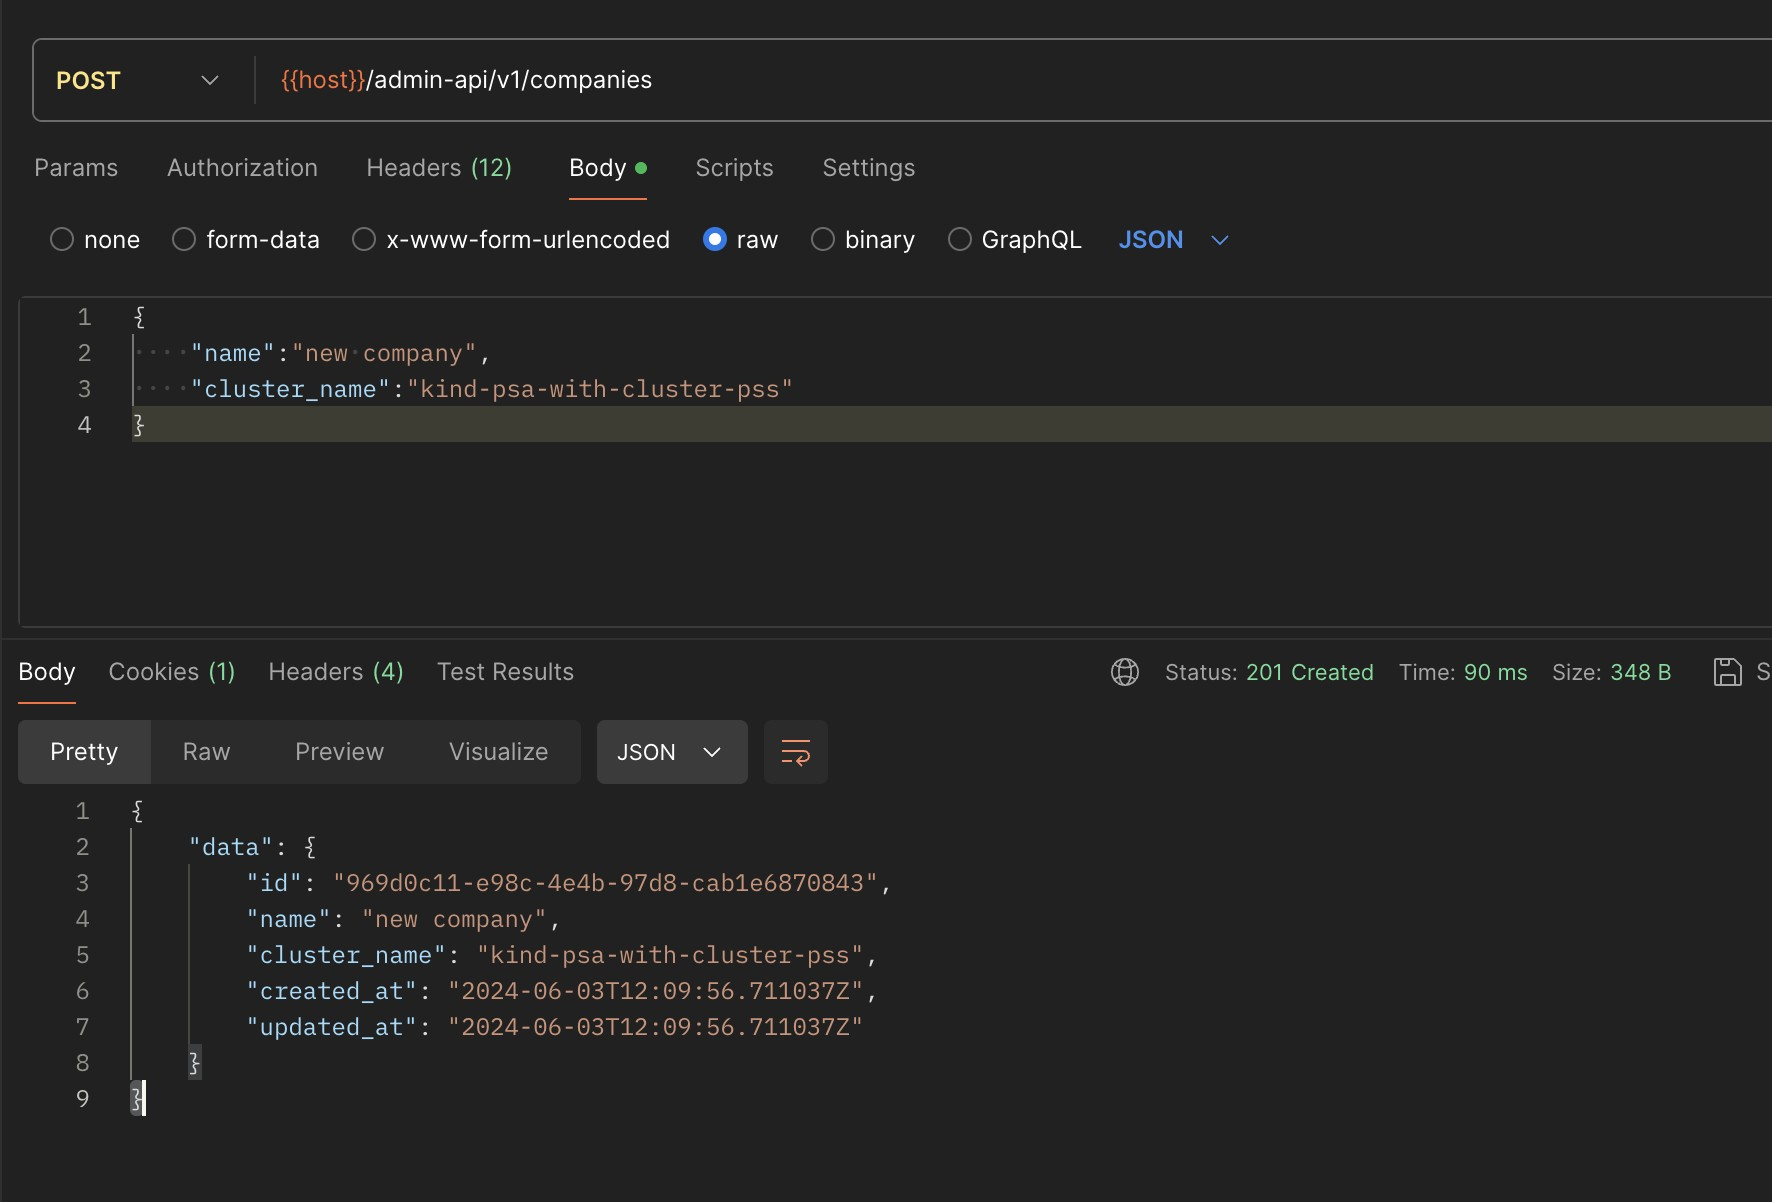
\includegraphics[width=0.8\textwidth]{resources/chapter-4/pengujian/p01.jpg}
  \caption{\textit{Request dan Response Pengujian} P01}
  \label{fig:pengujian-p01}
\end{figure}

Pengujian dengan ID P02 dilakukan dengan skenario yaitu admin tidak berhasil membuat \textit{company} karena nama cluster yang tidak tersedia pada server. Tersedia berarti, konfigurasi kubernetes cluster terdapat pada kubernetes \textit{config server} Admin akan membuat request dengan Postman kepada server dengan request seperti berikut.

\begin{enumerate}
  \item Mengisi \textit{field name} dengan nilai "new company"
  \item Mengisi \textit{field cluster\textunderscore name} dengan nilai "kind-psa-with-cluster-ps"
\end{enumerate}

\textit{Request} dibuat dengan membuat request menggunakan Postman pada url /admin-api/v1/companies dengan metode POST. \textit{request dan response} dapat dilihat pada gambar

\begin{figure}[ht]
  \centering
  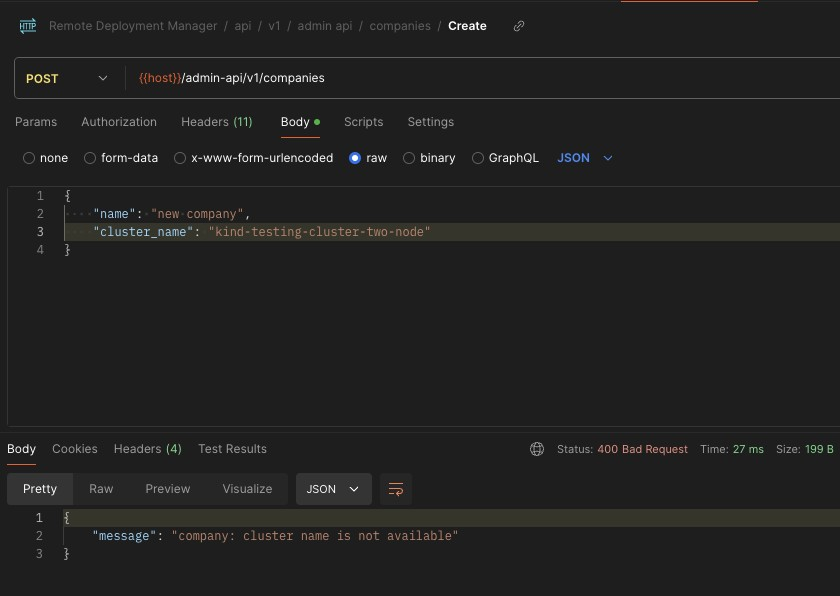
\includegraphics[width=0.8\textwidth]{resources/chapter-4/pengujian/p02.jpg}
  \caption{\textit{Request dan Response Pengujian} P02}
  \label{fig:pengujian-p02}
\end{figure}

Pengujian dengan ID P03 dilakukan dengan skenario yaitu admin ingin mendapatkan seluruh \textit{company} yang terdaftar pada sistem. Admin akan membuat GET request dengan Postman ke url /admin-api/v1/companies. Berikut merupakan balikan dari \textit{request} yang dikirimkan

\begin{figure}[ht]
  \centering
  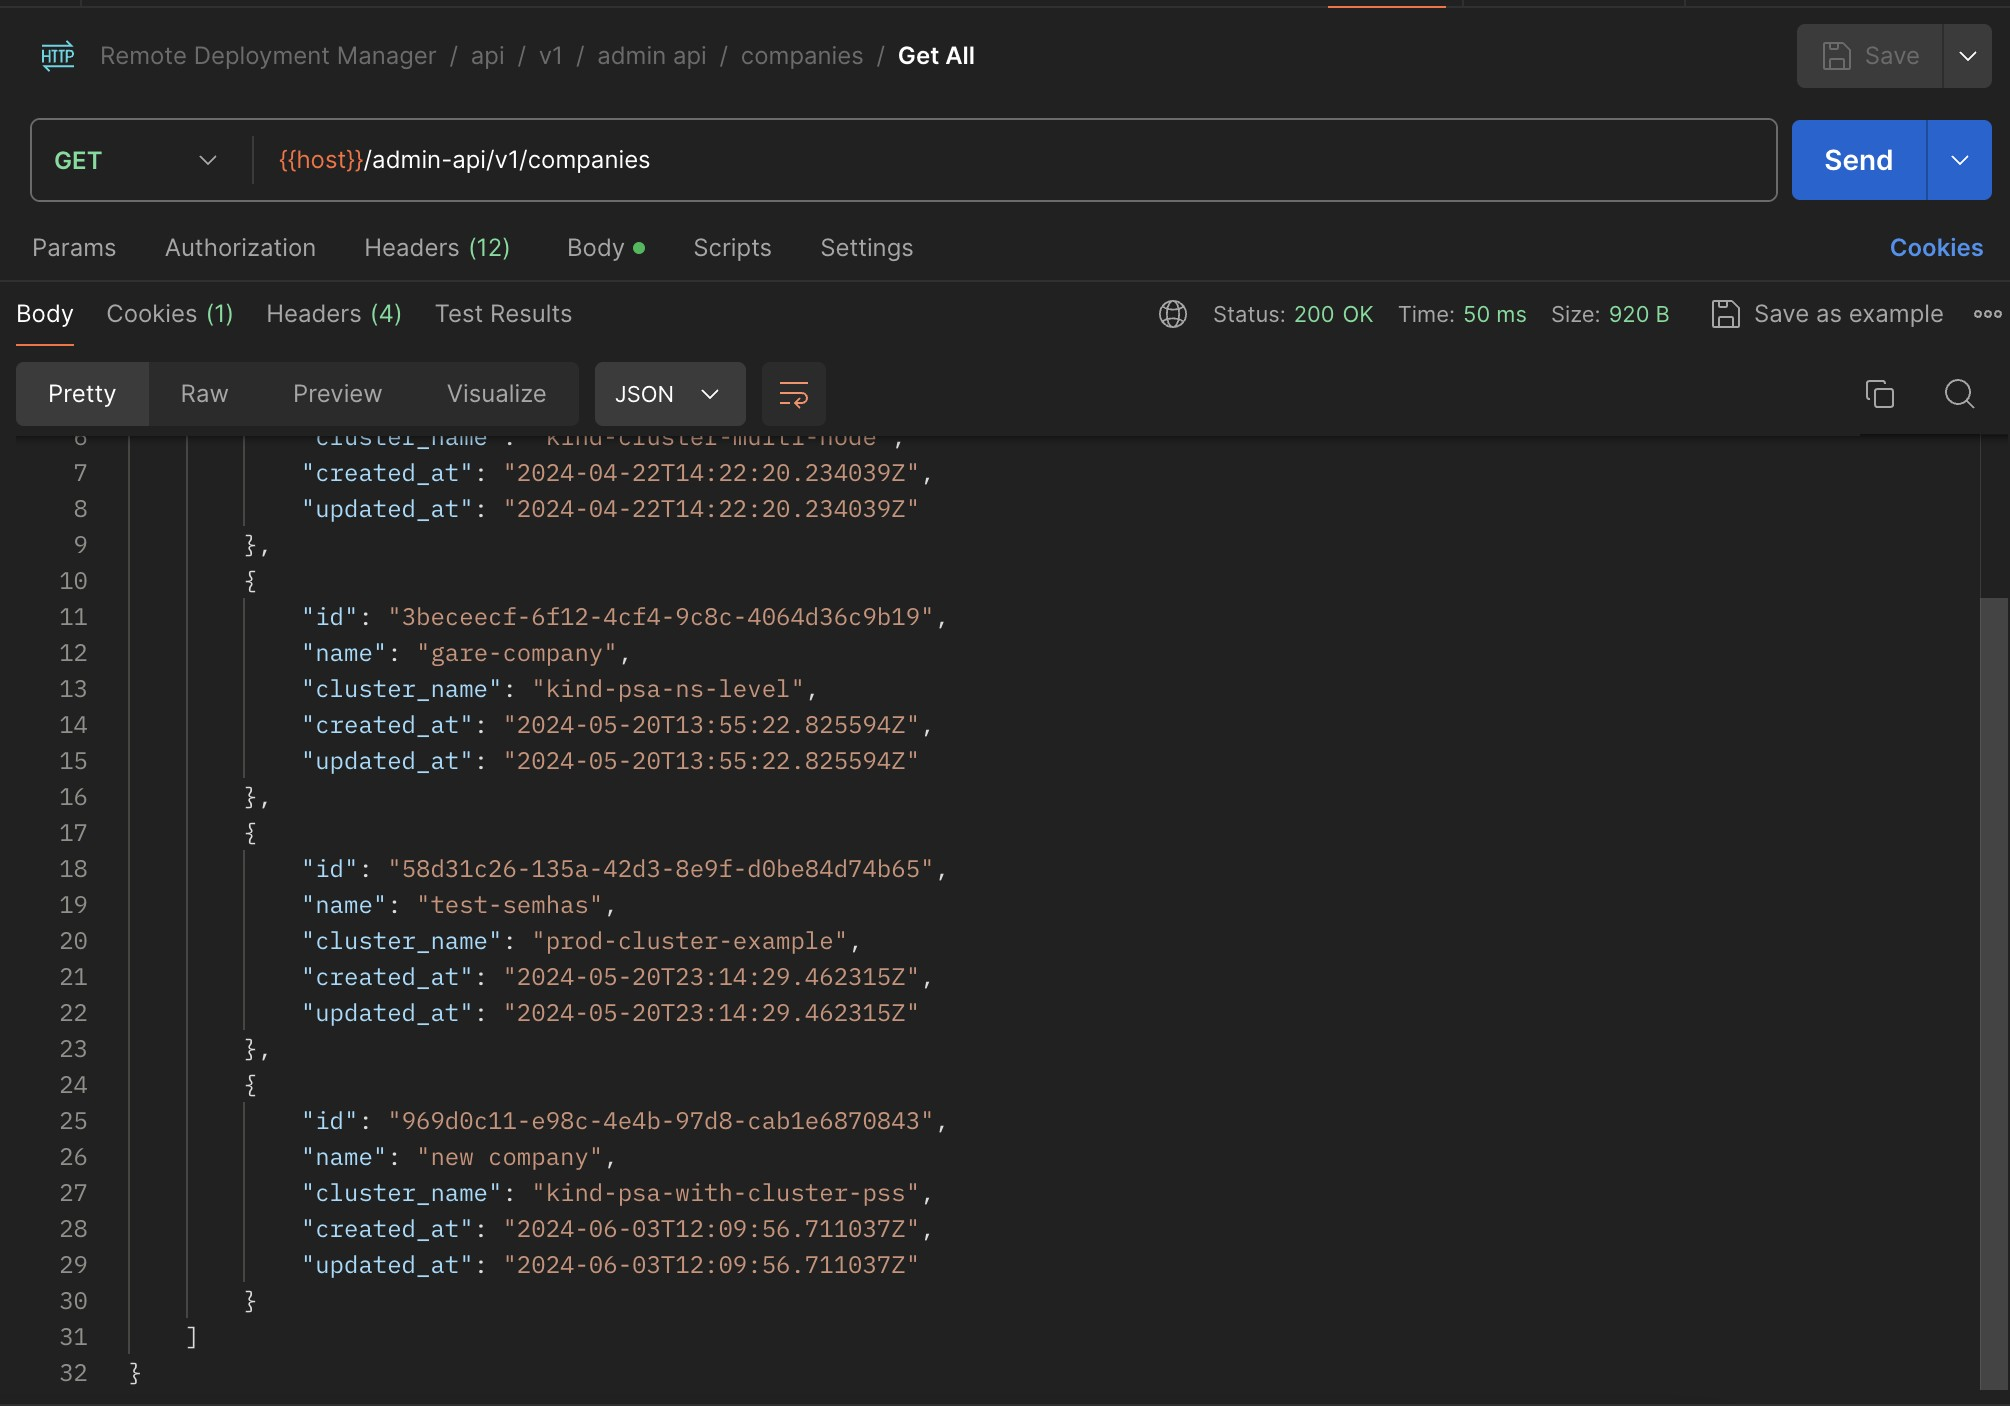
\includegraphics[width=0.8\textwidth]{resources/chapter-4/pengujian/p03.jpg}
  \caption{\textit{Request dan Response Pengujian} P03}
  \label{fig:pengujian-p03}
\end{figure}

Pengujian dengan ID P04 dilakukan dengan skenario yaitu admin ingin menghapus \textit{company} dengan id tertentu dari daftar \textit{company} pada sistem. Admin akan membuat DELETE request dengan Postman ke url /admin-api/v1/companies/:id. Admin menggunakan id company yang berhasil dibuat sesuai dengan gambar \ref{fig:pengujian-p01} sebagai parameter untuk \textit{company} yang dihapus. Berikut merupakan balikan dari \textit{request} yang dikirimkan.

\begin{figure}[ht]
  \centering
  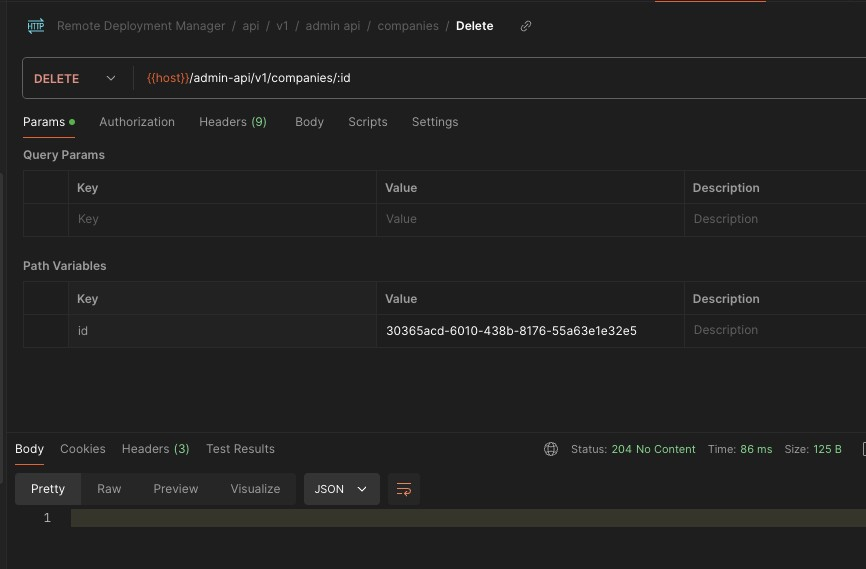
\includegraphics[width=0.8\textwidth]{resources/chapter-4/pengujian/p04.jpg}
  \caption{\textit{Request dan Response Pengujian} P04}
  \label{fig:pengujian-p04}
\end{figure}

Seluruh rekap pengujian pada domain \textit{company} dapat dilihat pada tabel .Berdasarkan hasil yang diperoleh, terbukti bahwa kebutuhan fungsional dengan ID tersebut telah terimplementasi dengan baik


\bgroup
\begin{table}[ht]
  \def\arraystretch{1.7}
  \caption{Skenario dan Hasil Pengujian Domain \textit{Company}}
  \label{tab:pengujian-domain-company}
  \centering
  \begin{tabular}{|p{2cm}|p{2cm}|p{3cm}|p{3cm}|p{2cm}|}
    \hline
    ID Fungsional & ID Pengujian                               & Skenario                                                                                                                                   & Ekspektasi & Realita \\
    \hline
    UC01          & Mendaftarkan perusahaan                    & Sistem memberikan akses kepada admin untuk mendaftarkan perusahaan yang ingin mendaftar ke dalam sistem                                                           \\
    \hline
    UC02          & Mendaftarkan \textit{user}                 & Sistem memberikan akses kepada admin untuk mendaftarkan \textit{user} ke perusahaan tertentu                                                                      \\
    \hline
    UC03          & Manajemen perusahaan                       & Sistem memberikan akses kepada admin untuk melakukan manajemen terhadap seluruh perusahaan yang terdaftar pada sistem                                             \\
    \hline
    UC04          & Manajemen \textit{user}                    & Sistem memberikan akses kepada admin untuk melakukan manajemen terhadap seluruh \textit{user} yang terdaftar pada sistem                                          \\
    \hline
    UC05          & Login                                      & Sistem memberikan akses kepada \textit{user}                                                                                                                      \\
    \hline
    UC06          & Melihat detail perusahaan                  & Sistem memberikan akses kepada \textit{user} untuk melihat perusahaanya                                                                                           \\
    \hline
    UC07          & Melihat \textit{user} pada satu perusahaan & Sistem memberikan akses kepada \textit{user} user lainnya pada satu perusahaan                                                                                    \\

    \hline
    UC08          & Manajemen \textit{perangkat}               & Sistem memberikan akses kepada \textit{user} untuk melihat, membuat, serta menghapus \textit{perangkat} yang terdaftar pada sistem                                \\
    \hline
    UC09          & Manajemen \textit{groups}                  & Sistem memberikan akses kepada \textit{user} untuk melihat, membuat, serta menghapus \textit{groups} yang terdaftar pada sistem                                   \\
    \hline
    UC10          & Manajemen \textit{deployment images}       & Sistem memberikan akses kepada \textit{user} untuk melihat, membuat, serta menghapus \textit{deployment images} yang terdaftar pada sistem                        \\
    \hline
    UC11          & Manajemen \textit{deployment plan}         & Sistem memberikan akses kepada \textit{user} untuk melihat, membuat, serta menghapus \textit{deployment plan} yang terdaftar pada sistem                          \\
    \hline
    UC12          & Melakukan \textit{Remote deployment}       & Sistem memberikan akses kepada \textit{user} untuk melakukan \textit{deployment} kepada target perangakt ataupun \textit{groups}                                  \\
    \hline
    UC13          & Melihat riwayat \textit{deployment}        & Sistem memberikan akses kepada \textit{user} untuk melihat riwayat \textit{deployment} yang telah dilakukan                                                       \\
    \hline
  \end{tabular}
\end{table}
\egroup


